This is the student profile page, accessible only from the topbar.\\
Here the student can view all his/her meetings that he/she has booked.\\
If the student wishes to delete a meeting, simply click on the blue box of the corresponding meeting.\\

\begin{figure}[H]
    \centering
     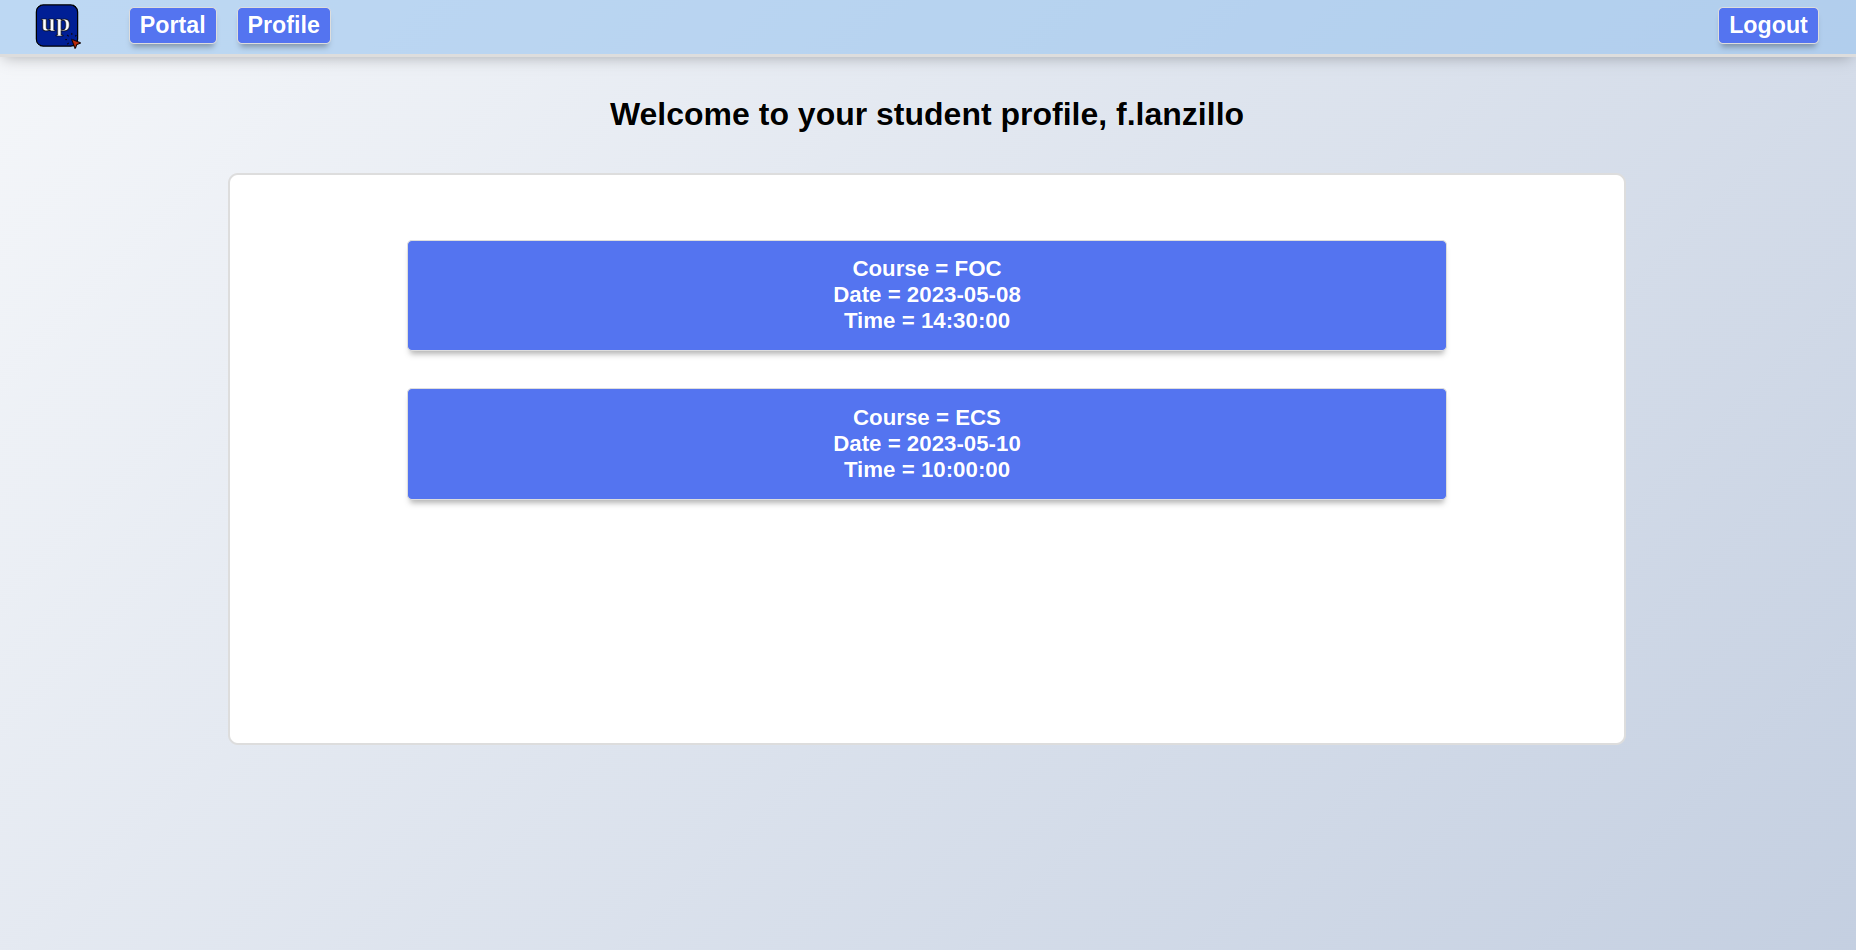
\includegraphics[width=0.95\textwidth]{img/user_manual/student/profile.png}
    \caption{\label{fig:student-profile-1} Screenshot of the student profile page.}
\end{figure}

Immediately after selecting the meeting to be deleted, an alert pops up and asks for the confirmation for the delete.\\
If the student wants to confirm he/she must click on the delete button otherwise on the x.\\

\begin{figure}[H]
    \centering
     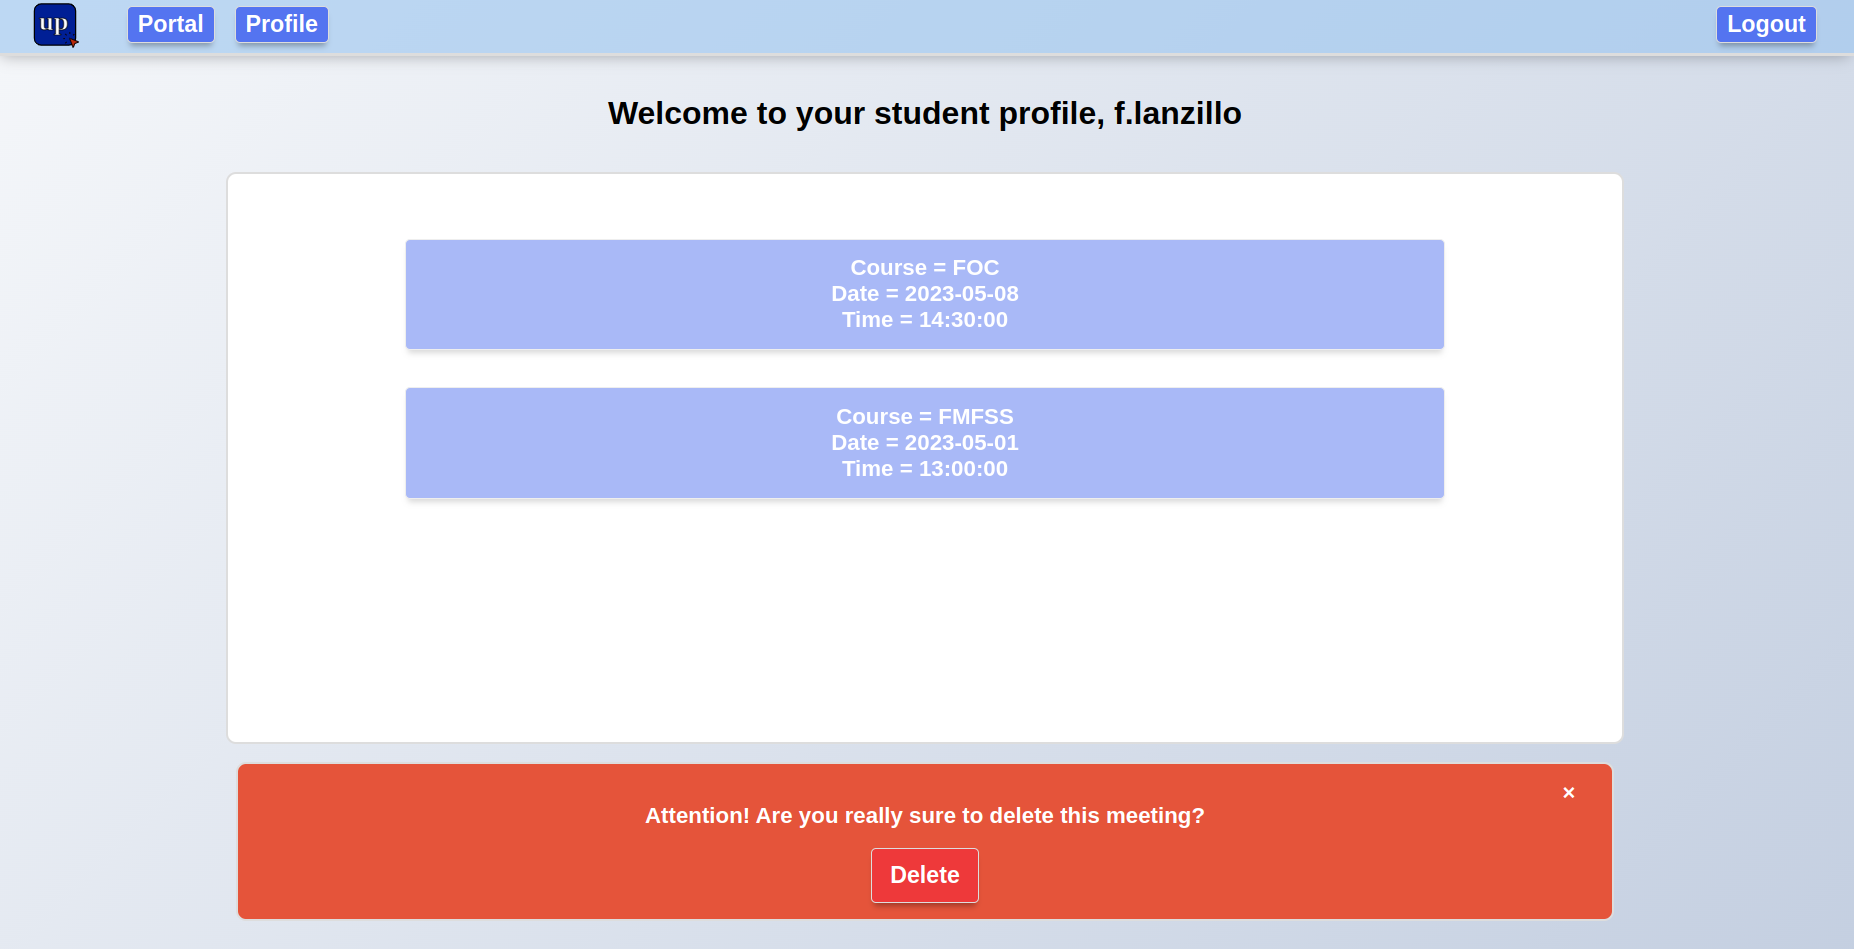
\includegraphics[width=0.95\textwidth]{img/user_manual/student/profile-delete-alert.png}
    \caption{\label{fig:student-profile-2} Screenshot of the delete alert of the student profile page.}
\end{figure}

The page shows a message with the result of the delete operation.\\

\begin{figure}[H]
    \centering
     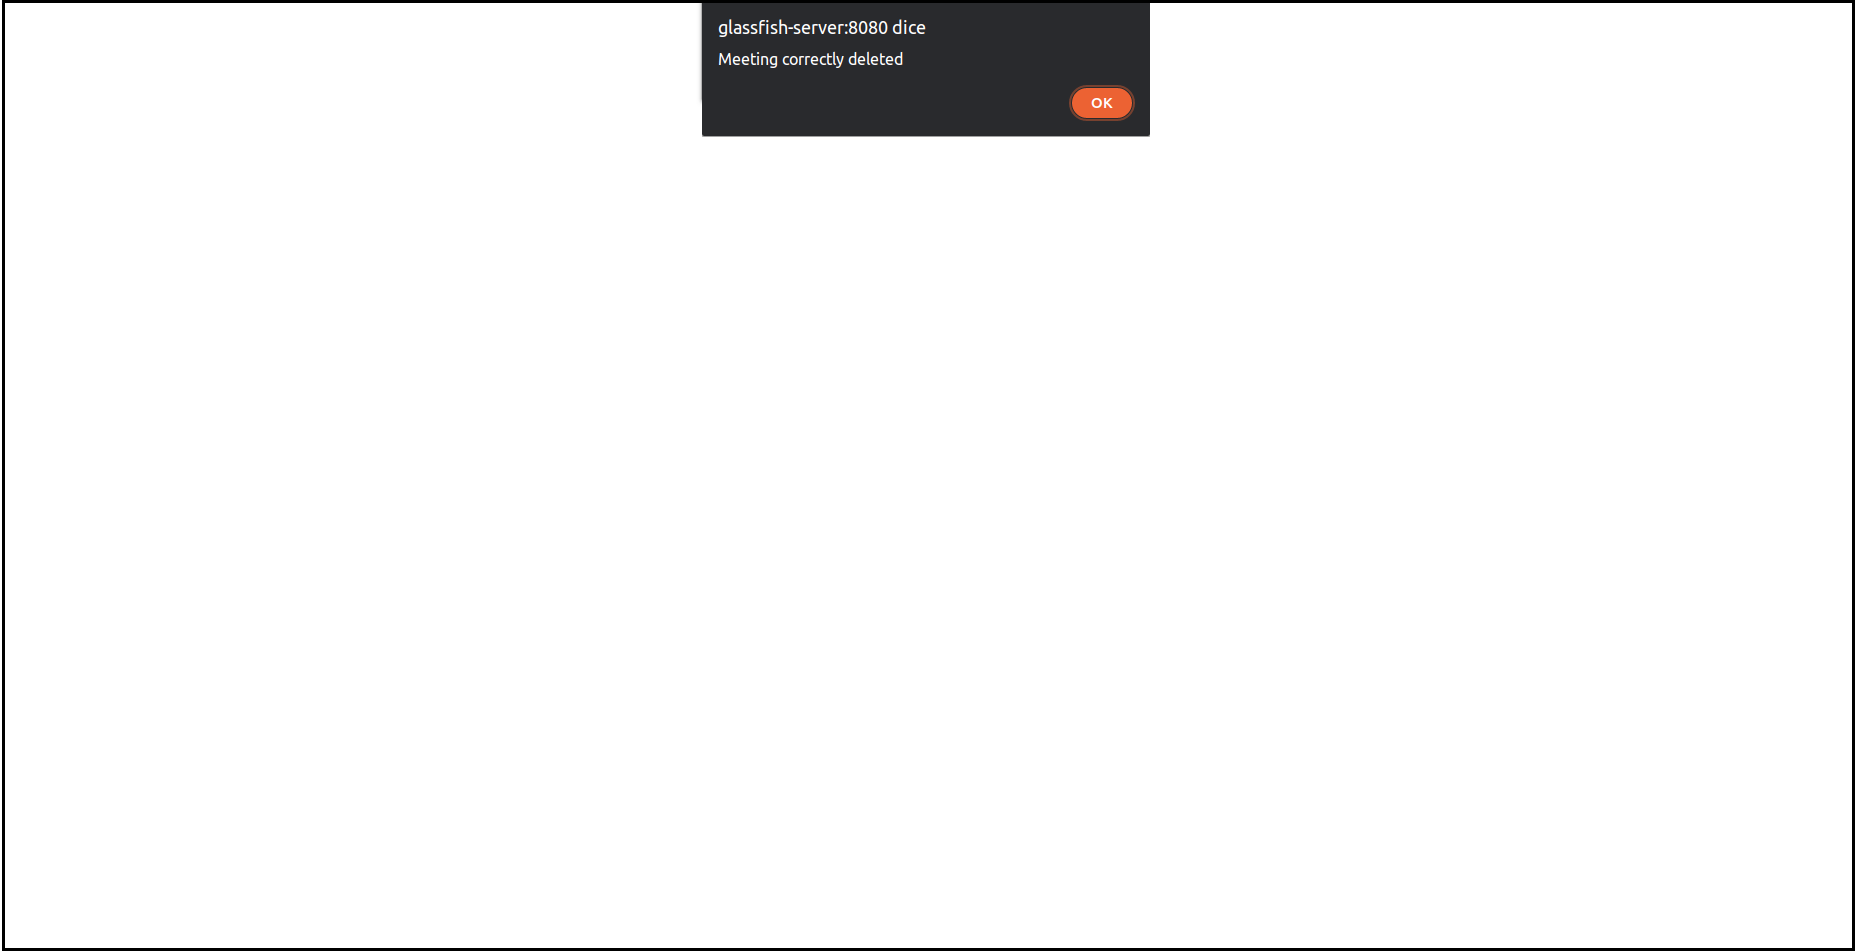
\includegraphics[width=1\textwidth]{img/user_manual/student/profile-alert.png}
    \caption{\label{fig:student-profile-3} Screenshot of the student profile page after the successful delete of the meeting.}
\end{figure}